\chapter{Les variables}
{ }\hfill\textbf{Niveau:} débutant\\ \\
\noindent \noindent Parfois, on souhaite tracer une figure à différentes échelles. Par exemple, si on souhaite dessiner un carré de côté 100, un carré de côté 200 et un carré de côté 50, actuellement on définirait trois procédures différentes correspondant à chacun de ces carrés. 
\begin{verbatim}
pour carre1
repete 4 [av 100 td 90]
fin
pour carre2
repete 4 [av 200 td 90]
fin
pour carre3
repete 4 [av 50 td 90]
fin
\end{verbatim}
On s'aperçoit immédiatement qu'il serait plus simple de définir une seule procédure à laquelle on préciserait juste la longueur du côté à tracer. Par exemple, \texttt{carre 200} tracerait le carré de côté 200, \texttt{carre 100} tracerait le carré de côté 100 etc. C'est précisément ce que vont permettre de réaliser les variables.
\section{Exemples d'utilisation}
\noindent Pour tracer un carré de côté 100, on utilise:
\begin{verbatim}
pour carre
repete 4[av 100 td 90]
fin
\end{verbatim}
Nous allons modifier cette procédure afin qu'elle reçoive un paramètre (on dit également \og argument \fg) indiquant la longueur du côté à tracer. \\
Un nom de variable est toujours précédée du symbole \og : \fg. Lorsqu'on veux indiquer que la procédure \texttt{carre} dépend de la variable \texttt{:c}, on rajoute \texttt{:c} à la fin de la ligne de défnition. \\
Par conséquent, ensuite, on avancera non plus de 100 pas de tortue mais de \texttt{:c} pas de tortues. La procédure devient alors:
\begin{verbatim}

pour carre :c
repete 4[av :c td 90]
fin
\end{verbatim}
Ainsi, en tapant: \texttt{carre 100 carre 50 carre 30 carre 20 carre 10}\\
 \begin{center}
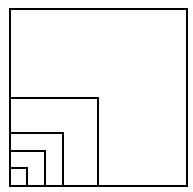
\includegraphics[scale=0.5]{images/variables-carres.png}
\end{center}
 \vspace{1cm}
 \section{Tracer un rectangle de longueur et largeur déterminée}
 \noindent On définit ici une procedure nommée \texttt{rec} qui dépend de deux variables représentant les deux dimensions du rectangles. \texttt{rec 200 100} trace ainsi un rectangle de hauteur 200 et largeur 100.
 \begin{verbatim}
pour rec :lo :la
repete 2[av :lo td 90 av :la td 90]
fin
\end{verbatim} 
Faites des essais: 
\begin{verbatim}
rec 200 100 rec 100 300 rec 50 150 rec 1 20 rec 100 2 
\end{verbatim}
Bien sûr, si vous ne donnez qu'un argument à la procédure \texttt{rec}, l'interpréteur vous signalera par un message d'erreur que la procédure attend un autre argument.
\section{Tracer une forme à des tailles diverses}
\noindent
Nous avons vu comment tracer un carré, un rectangle à des tailles différentes. Nous allons reprendre l'exemple de la maison p. \pageref{maison} et voir comment modifier le code pour tracer la maison à l'échelle souhaitée.\\ \\
L'objectif est de passer un argument à la procédure \texttt{ma} pour que selon le paramètre, la maison soit plus ou moins grande. Nous souhaitons que \texttt{ma 1} trace la maison en taille réelle.\\
\texttt{ma 0,5} tracera une maison à l'échelle 0,5. \\
\texttt{ma 2} tracera une maison aux dimensions deux fois plus grandes etc \\ \\
La notion de proportionnalité est bien sûr sous-jacente. En vraie grandeur, la procédure \texttt{carre} était la suivante:
\begin{verbatim}
pour carre 
repete 4[av 150 td 90]
fin
\end{verbatim}
Toutes les dimensions originales de la maison sont multipliées par l'échelle. La procédure \texttt{carre} devient: 
\begin{verbatim}
pour carre :c
repete 4[av 150*:c td 90]
fin
\end{verbatim}
Ainsi quand on tapera \texttt{carre 2}, le carré aura pour côté $150\times2=300$. les proportions sont bien respectées! En fait, on s'aperçoit qu'il va juste falloir reprendre toutes les procédures et changer les longueurs de déplacement de la manière suivante: \\
\texttt{av 70} devient \texttt{av 70*:c} \\ 
\texttt{av 45} devient \texttt{av 45*:c} \\
etc\\ \\
\begin{verbatim}
pour carre :c
repete 4[av 150*:c  td 90]
fin

pour tri :c
repete 3[av 150*:c td 120]
fin

pour porte :c
repete 2[av 70*:c td 90 av 50*:c td 90]
fin

pour che :c
av 55*:c td 90 av 20*:c td 90 av 20*:c
fin

pour dep1 :c
td 90 av 50*:c tg 90
fin

pour dep2 :c
tg 90 av 50*:c td 90 av 150*:c td 30
fin

pour dep3 :c
lc td 60 av 20*:c tg 90 av 35*:c bc
fin

pour ma :c
carre :c dep1 :c porte :c dep2 :c tri :c dep3 :c che :c
fin
\end{verbatim}
\section{Exercice:}
\noindent Réaliser les dessins suivants avec des variables de telle sorte que l'on puisse les obtenir à des tailles diverses.\\ \\ \\
\begin{center}
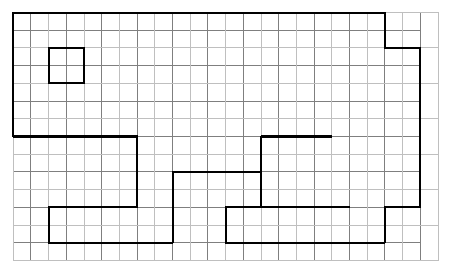
\includegraphics[scale=0.7]{images/variables-grenouille.png}
\end{center}
\begin{center}
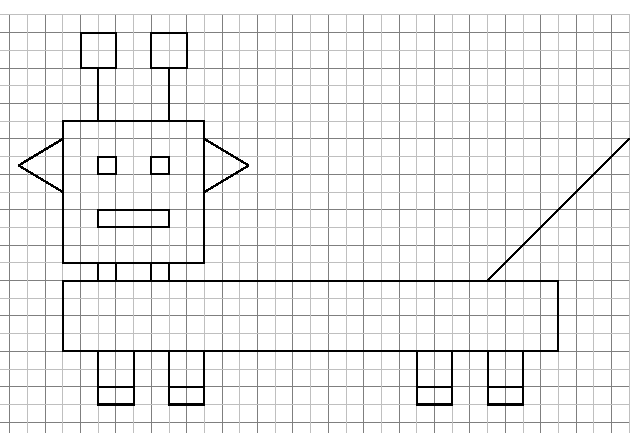
\includegraphics[scale=0.75]{images/variables-robot.png}
\end{center}
